\chapter{Learned Quantization\label{cha:chapter3} Schemes}
\hspace*{1em}This chapter introduces two custom learned quantization schemes — approaches that allow models to learn to quantize
with adjustable intensity. The first one, a custom quantization layer featuring a threshold for gradient-based scale updates,
will be discussed in \cref{sec:nestedquantizationlayer}. The second scheme, which focuses on custom regularization terms with a configurable penalty rate,
will be covered second in \cref{sec:customloss}.

% ------------------------------------------------------------
% ----------------------- learnedquantization Schemes ----------------------- 
% ------------------------------------------------------------

\section{Nested Quantization Layer}
\label{sec:nestedquantizationlayer}
\hspace*{1em}To separate the quantization logic from the usual structure of NN layers,
we define a nested quantization layer that can be used within a standard one. 
This approach provides usability, making it easy to extend the functionality to other types of layers beyond dense and convolutional ones.
We will first explain the core logic of the nested quantization layer and how it integrates into a model,
followed by a detailed explanation of how the trainable scaling factors are updated.


% -------------------- Implementation details --------------------

\subsection{Core Logic and Structure}
\label{subsec:corelogicandstructure}

\hspace*{1em}As the name "nested quantization layer" suggests —
this layer is implemented in a way that it is initialized from within a model layer itself.
To explain, let \( P \) be the parameters of a layer (weights, bias or kernel). This \( P \) is used
as the input for the nested quantization layer, where it undergoes quantization based on 
a scaling factor \( s \). In turn, \( s \) is the only trainable parameter of the nested layer itself.
The forward-pass of the nested layer performs the following operation:
\[
  P_{reconstructed} = P_{quantized} \cdot s
\]
where \( P_{quantized} \) is the quantized integer form of \( P \) and is defined as:
\[
  P_{\text{quantized}} = \left\lfloor \frac{P}{s} \right\rfloor
\]
During back-propagation, the nested layer receives the upstream gradient of
\( P_{reconstructed} \) and passes it downward as is.  This follows the standard STE behaviour
used with non-differentiable discretizers, such as \(  \lfloor \cdot \rfloor\) in our case,
as discussed in \cref{subsec:commonquantizationapproaches}.

For updating the scale factor \( s \) — its own trainable parameter — 
the nested layer utilizes the upstream gradient of \( P_{\text{reconstructed}} \)
and applies a custom logic, which will be detailed in \cref{subsec:learnedscalefactor}. 
Essentially, this approach solves two problems with one tool — updating both 
\( P \) and \( s \) using the same gradient, though with different logic.

Conceptually, the resulting structure with one or more nested quantization layers is illustrated in \cref{fig:nested_quantization}
on the example of a convolutional layer.

\begin{figure}[h!]
  \centering
  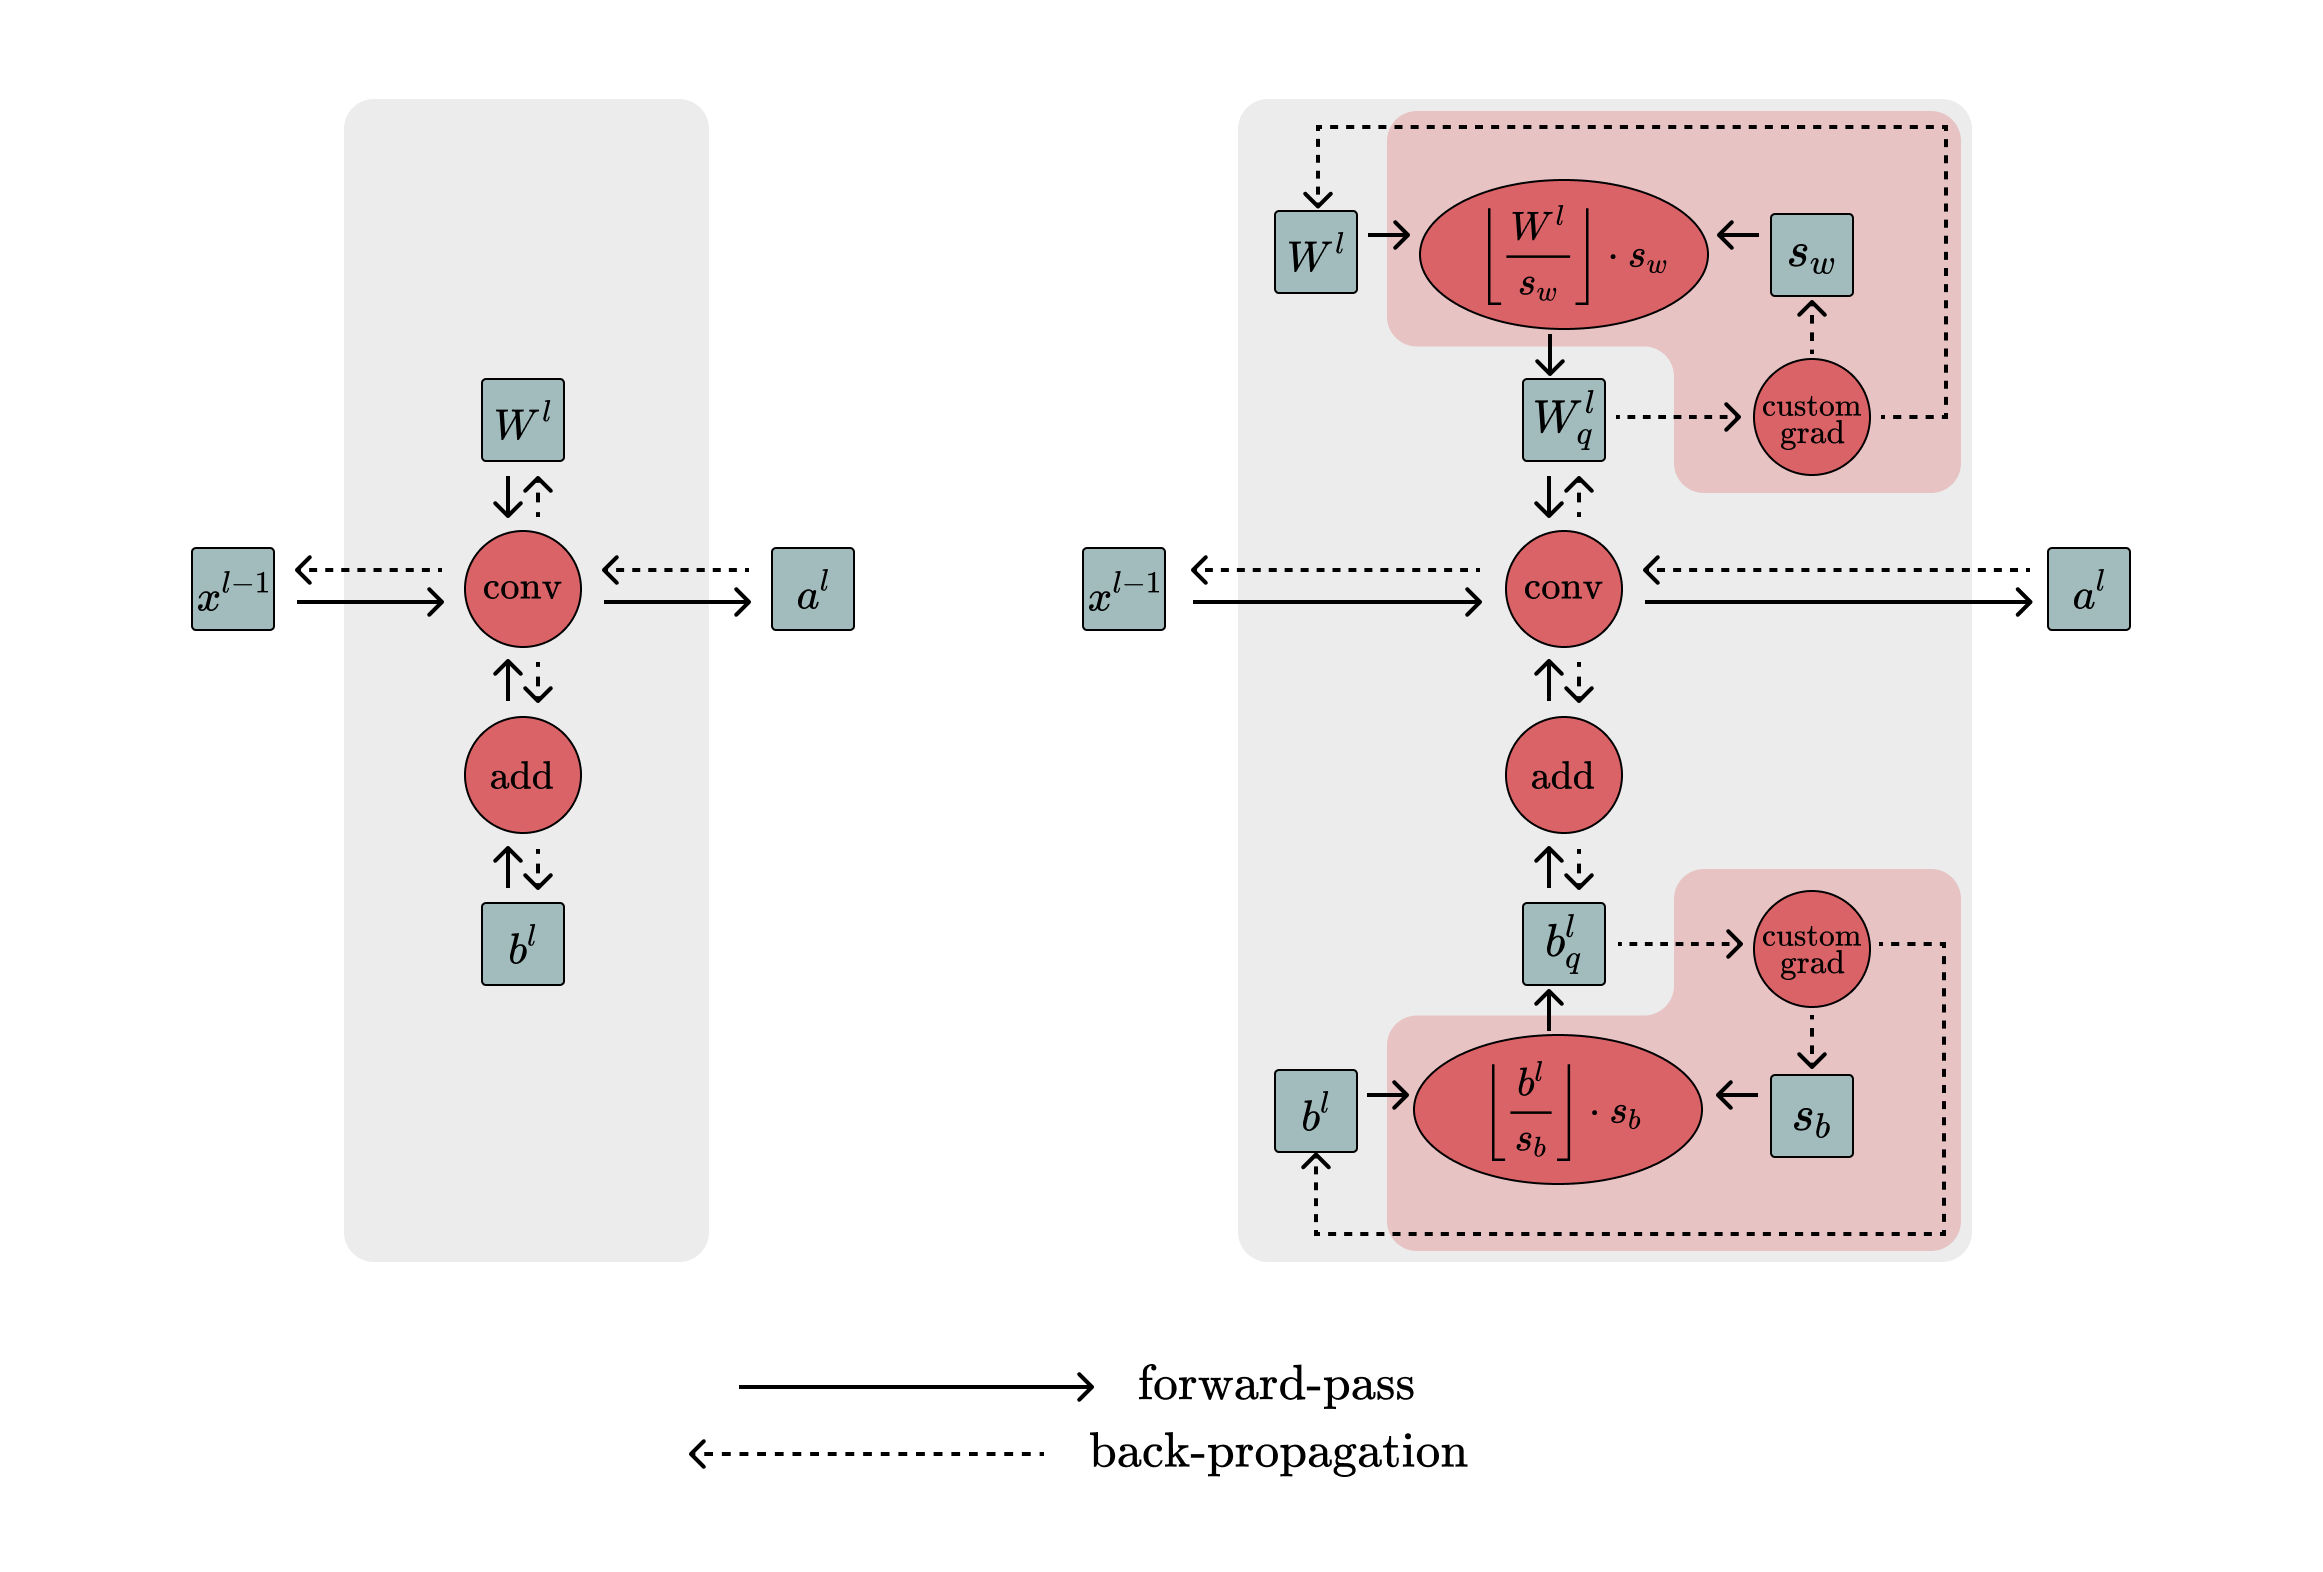
\includegraphics[width=14cm]{nested_quantization_layer.png}
  \caption{A convolutional layer (left) and its integration with the nested quantization layer (right) for both weights and bias.
  Trainable scaling factors are updated using custom gradients. Parameter gradients are passed downward as is.}
  \label{fig:nested_quantization}
\end{figure}

Since the scaling factor \( s \) can have different shapes and be applied at varying levels of granularity,
we have enabled scalar, row-wise, and column-wise application granularity for dense layers,
as shown in \cref{fig:scaler-application-dense}. 
For convolutional layers, we additionally support channel-wise granularity,
corresponding to the first four scenarios in \cref{fig:granularity-conv2d}.

\begin{figure}[t!]
  \centering
  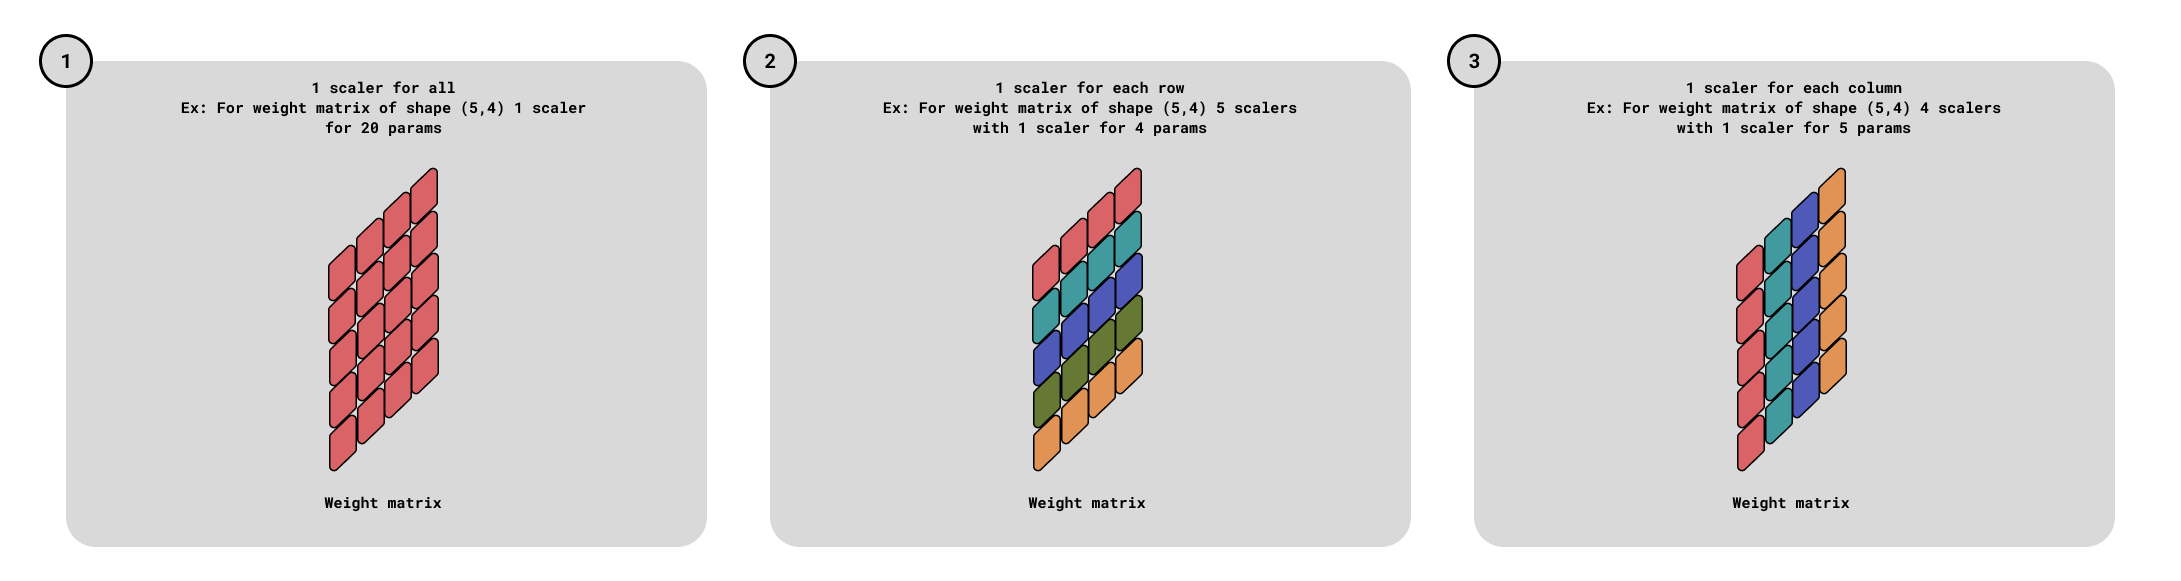
\includegraphics[width=14cm]{Scaler-application-dense.png}
  \caption{Various applications of scaling factors, ranging from a single scalar applied to the entire weight matrix (1) to row-wise and column-wise application of vector scalers.}
  \label{fig:scaler-application-dense}
\end{figure}

The nested layer is built upon Tensorflow's \texttt{tf.keras.Layer} class,
which serves as the base for all Keras layers. The gradient calculation logic is wrapped
in Tensorflow's \texttt{tf.custom\_gradient} decorator, allowing proper functioning of the 
model's computational graph. Dense and convolutional layers have been implemented as 
\texttt{tf.keras.Layer} objects with minimal adjustments as well to incorporate the nested layers logic.

% -------------------- concept and design --------------------

\subsection{Learned Scale Factor}
\label{subsec:learnedscalefactor}

\hspace*{1em}For the trainable scale factor \( s \), we define a custom gradient formula. 
The gradient of the loss with respect to \( s \), denoted as \( \nabla_s L \), is computed as:
\[
\nabla_s L = g_s \cdot m
\]

Let us consider both multiplication terms separately. \(  g_s  \) is the main "decision maker" on whether to
increase the scale and, therefore, quantize more. \(  g_s  \) is
calculated using a hyperparameter threshold  \(  \lambda  \),
which is compared against the ratio \(  r  \).
\[
g_s = 
\begin{cases} 
0, & \text{if } r \geq \lambda \\
- \tanh(\lambda - r), & \text{if } r < \lambda
\end{cases}
\]

In turn, \(  r  \) is the ratio between the upstream gradient of the layer's reconstructed parameter \( P_{reconstructed}\) 
with respect to the loss
and its absolute value (for simplicity, we denote \( P_{reconstructed}\) as \(P_r\)):
\[
r = \frac{\left| \nabla_{P_{r}} L \right|}{\max(\epsilon, \left| P_r \right|)}
\]

The formula conveys the relative impact of the gradient on the parameter's value.
A large \(  r  \) indicates that the parameter is not ready for intense quantization
because small perturbations can lead to significant changes in its optimization.
Conversely, parameters with a small \(  r  \) are better candidates
for quantization since they are less sensitive.

The decision to replace \( P_r \) with \( \epsilon \) when \( P_r = 0 \)
ensures that the corresponding \( r \) becomes large,
effectively resisting quantization. This behavior is valid regardless of the parameter's sensitivity
 — if the zero parameter is sensitive, quantization could disrupt future optimization steps,
 and if it is not sensitive, quantization adds no value since \( s \) has a positive non-zero constraint 
 and \( \frac{P}{s} \) will remain zero.

The motivation behind using \( tanh(\cdot) \) primarily stems from two key reasons. 
First, \( tanh(\cdot) \) is bounded (in our use case, to \( [-1, 0) \)), 
which prevents excessive gradient magnitudes.
Second, unlike sigmoid, the hyperbolic tangent does not require any additional rescaling since it is
symmetric around \( 0 \). An additional point is that \( tanh(\cdot) \) saturates comparably faster than the sigmoid function,
potentially allowing for more decisive gradients,
but it is uncertain how much influence this has.

Now that \( g_s \) is covered, let's take a look at \( m \) defined as:
\[
m = \max\left(\left| P_{\text{quantized}} \right|\right) 
\]
where the shape of \( m \) corresponds to the shape of \( s \).
For example, if \( s \) is a row-wise scaler, then \( m  \) will hold
the maximum value from each row of \( \left| P_{quantized} \right|\).
Similarly if  \( s \) is a single scalar value, then \( m \) represents
the maximum across the entire layer parameter.

A larger \( m \) indicates a wider range of quantized values,
implying the parameter can tolerate coarser quantization.
In contrast, a smaller \( m \) means a narrower range,
where intense quantization could be rather harmful.
As a result, by multiplying \( g_s\) with \( m \), 
the adjustment to the scale becomes proportional to the parameter's range.
This encourages coarser quantization for parameters with larger ranges
while being conservative for smaller ones.

To sum this part up, the intuition is that the gradient adjustment for the scale factor
\( s \) adapts dynamically based on both the sensitivity of the parameter  \( g_s\) 
and its range \( m \) . Sensitive parameters are left with a "zero vote",
while the less sensitive ones have a say on how much quantization they can tolerate.

In cases where all parameters are deemed sensitive with \( r \geq \lambda\) and
\( g_s =  0 \), the scale factor \(s\) does not receive gradient updates.
Such a situation could result in an unfavorable outcome
where the parameters themselves increase in magnitude while the scale factor remains unchanged,
loosening the achieved quantization.
To address this, we apply a small constant update tied to \( \lambda \) in cases where 
all parameters have \( r \geq \lambda\). As a result, the initial formula for \( g_s\) becomes:
\[
g_s = 
\begin{cases} 
- \tanh(\lambda), & \text{if } \forall P_r, \, r \geq \lambda \\
- \tanh(\lambda - r) \cdot \mathbf{1}(r < \lambda), & \text{otherwise}
\end{cases}
\]

Finally, the scale gradients are initially calculated for each parameter value
but are then aggregated along the corresponding granularity axes.
This aggregation reflects the collective behavior of parameters within the same granularity,
where only those deemed quantizable and with a meaningful "say" contribute to the overall adjustment,
while sensitive parameters express their resistance with a "zero vote".
Even when all parameters are sensitive and each casts a "zero vote", 
we still force the "elections" by introducing a constant gradient term
to avoid stagnation in scale factor updates.

In \cref{cha:chapter4}, we will present experimental results for different values of 
\( \lambda \), offering guidance on the optimal values for both dense and convolutional layers.

% ------------------------------------------------------------
% ----------------------- custom loss functions ----------------------- 
% ------------------------------------------------------------

\section{Custom Loss Function Terms}
\label{sec:customloss}
\hspace*{1em}Building on the nested quantization layers covered in \cref{sec:nestedquantizationlayer},
we define three custom loss function terms that can be used in combination with the task-specific loss.
We will first explain how these terms fit into the model's structure and training process,
then provide the details of their individual formulations.

% --------------------  --------------------
\subsection{Design and Integration}
\label{subsec:designandintegration}
To incorporate custom loss terms into the model's training process,
we utilize the nested layers described in \cref{sec:nestedquantizationlayer}, with a slight modification.
The modification lies in the gradient calculation of the nested layers,
where we similarly use STE for parameter updates, but do not provide any gradient updates for the scale factors altogether.
This is equivalent to setting \( \lambda = 0\), which disables gradient updates for the scale factors.

Instead, to update scale factors, we define a custom loss term \( \mathcal{L}_{custom}\) scaled by a penalty rate \( \gamma \),
an adjustable hyperparameter. This loss term depends on the model parameters and scale factors
and is added to the task-specific loss:
\[
\mathcal{L}_{\text{total}} = \mathcal{L}_{\text{task}} + \gamma \cdot \mathcal{L}_{\text{custom}}
\]

As visualized in \cref{fig:custom_loss_term_integration}, 
scale factors receive gradient updates from the custom loss term,
while the gradients for model parameters are influenced by both the task-specific loss
and the custom loss term. To illustrate this process further,
if we set \( \gamma = 0 \), the scale factors will not receive any updates,
and the model will rely on the STE to adapt to the initial values of the scale factors during training.

\begin{figure}[t!]
  \centering
  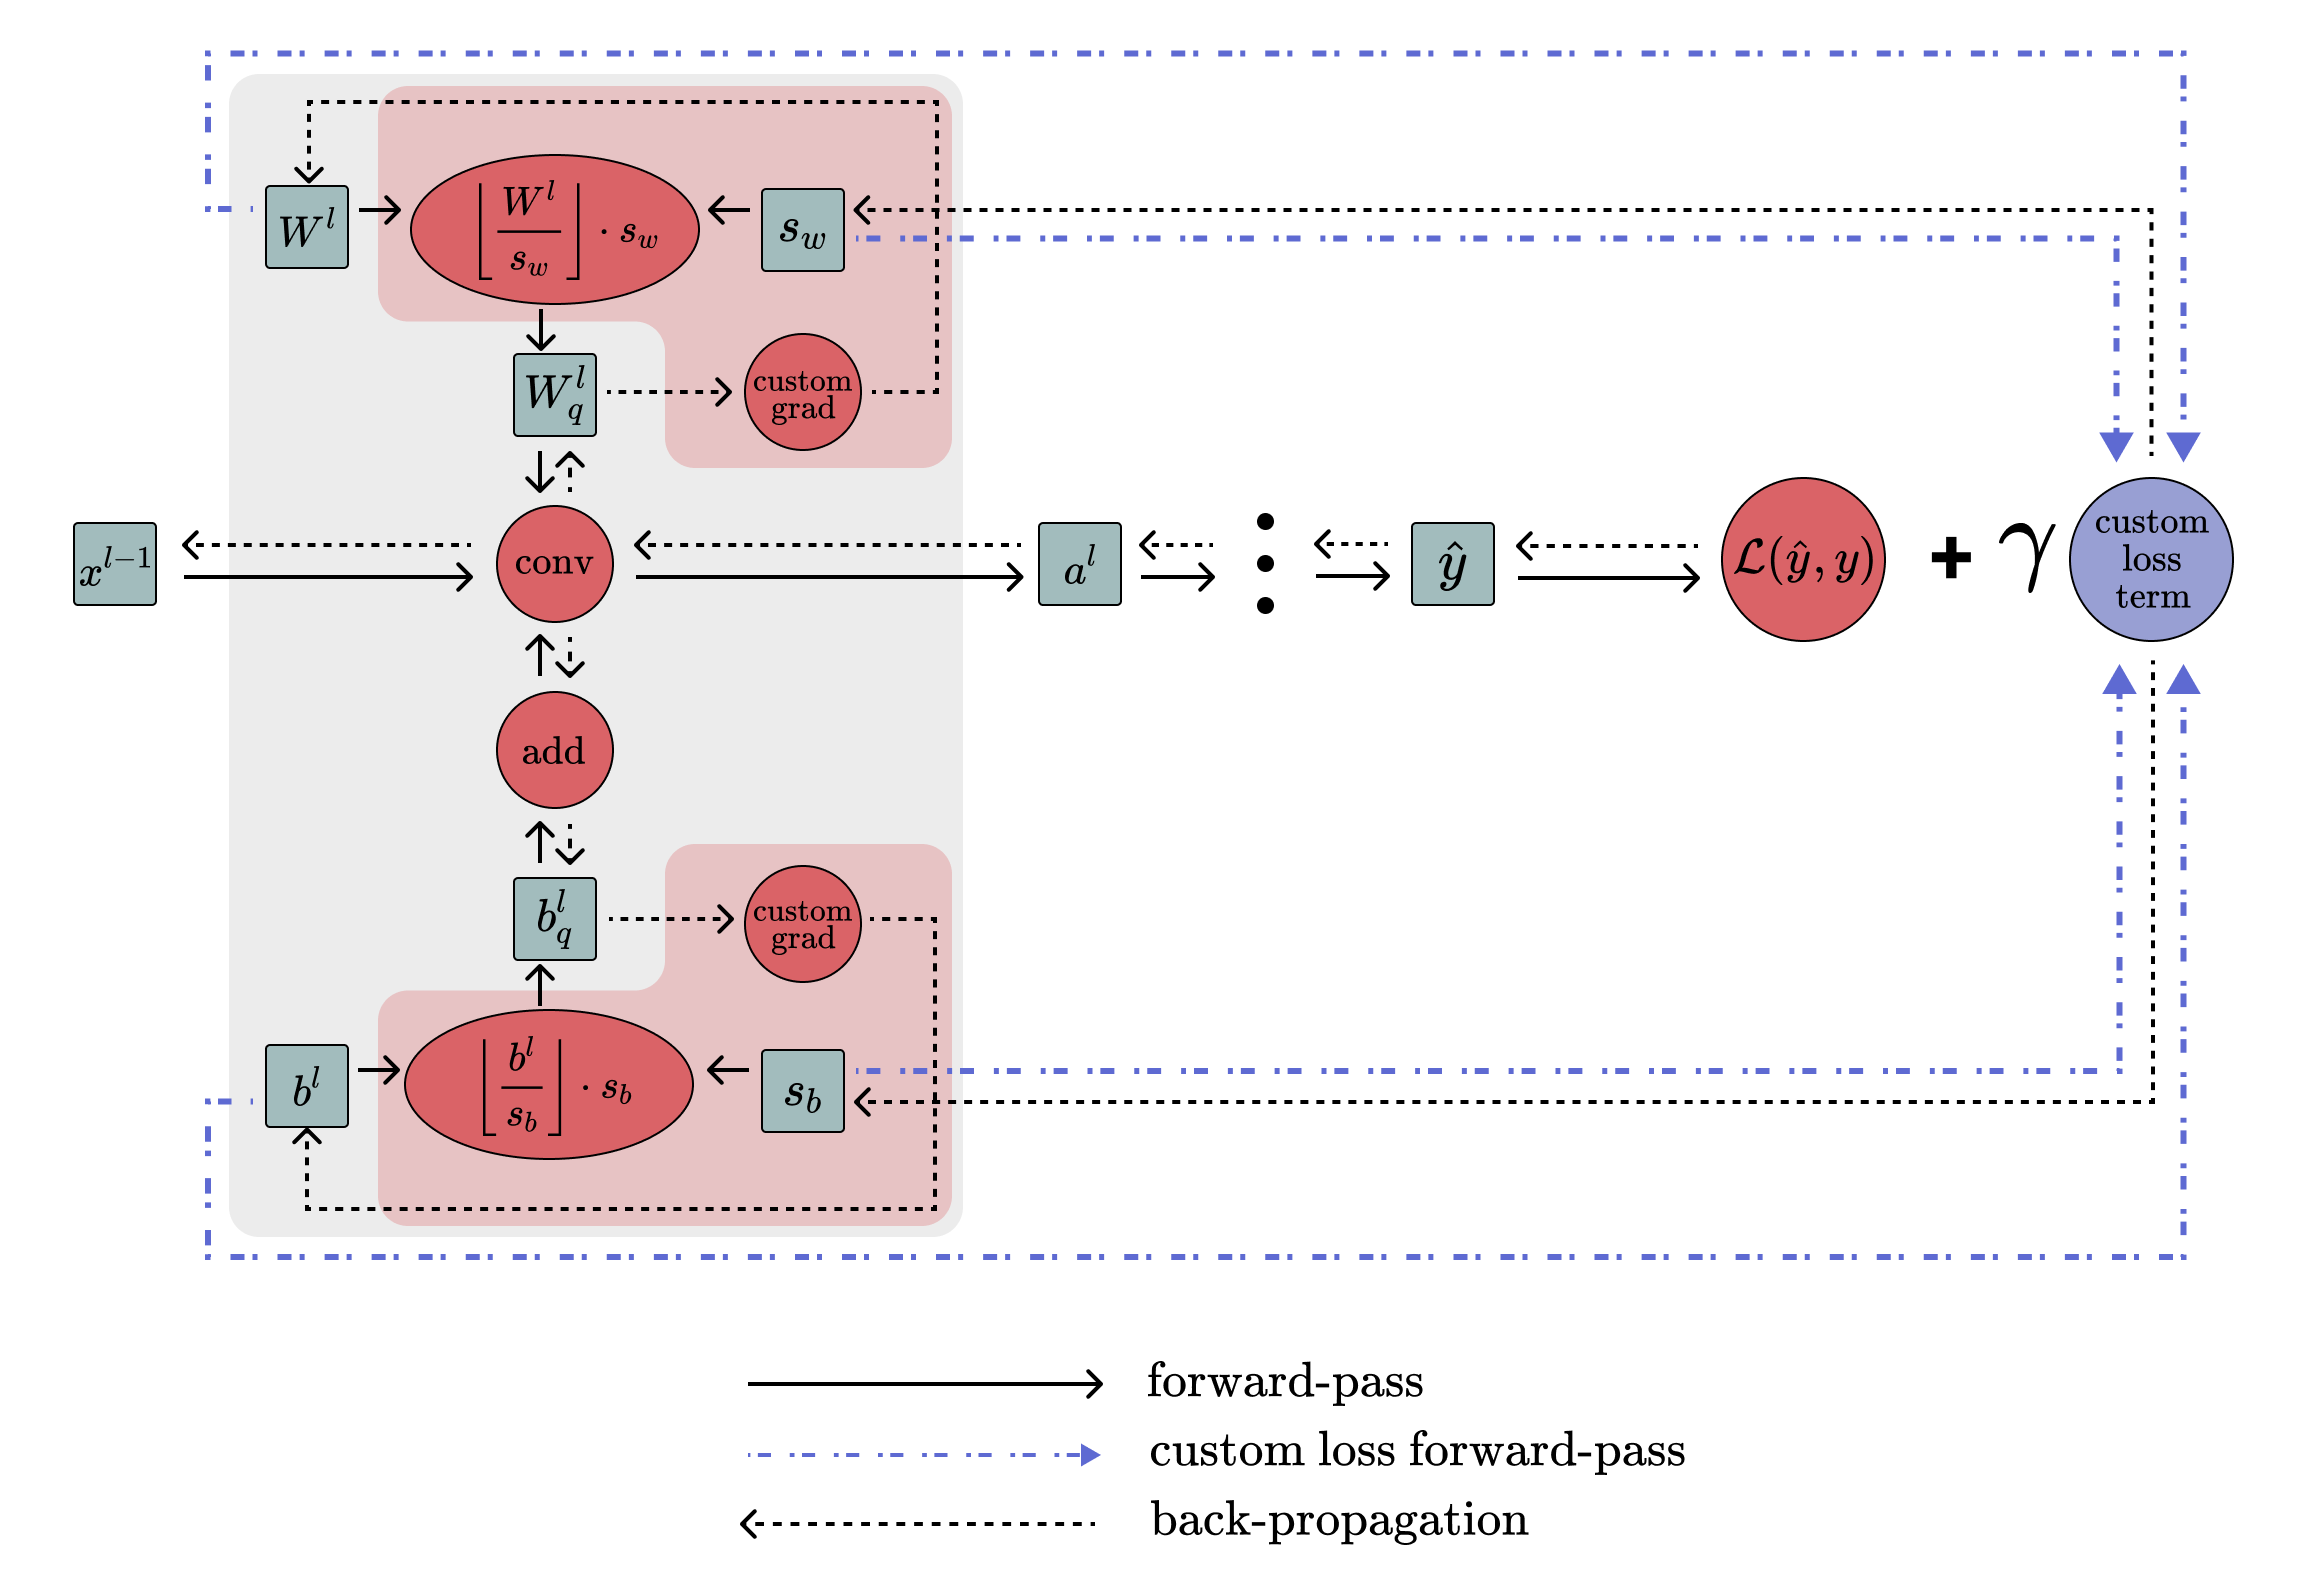
\includegraphics[width=14cm]{custom_loss_term_integration.png}
  \caption{Custom loss term using scale factors and model parameters integrated into training.}
  \label{fig:custom_loss_term_integration}
\end{figure}

The custom loss terms are implemented as Python objects
to which the model's nested quantization layers are passed.
These objects have access to the latest values of parameters
and scale factors at any point during training.

Unlike the method described in \cref{sec:nestedquantizationlayer},
this approach defines a forward-pass to calculate the custom loss terms,
rather than manipulating gradients directly.
As a result, it may appear more straightforward
and will be shown to achieve equally good results..

% -------------------- Loss component definitiona --------------------
\subsection{Loss Term Definitions}
\label{subsec:losstermdefinitions}

\hspace*{1em} We use the same notation, 
with \( P \) representing the parameters of a nested quantization
layer (weights, bias or kernel) and \( s \) as the corresponding scale factor.
Additionally, we denote the elements in the scale factor \( s \) as \( \{ s_1, \dots, s_K \} \).

\textbf{MaxBin Penalty.} We name the first custom loss term MaxBin Penalty and
define the function \( \text{maxbin}(P, s) \) 
as the collection of per-\( s_k\) maxima:
\[
\text{maxbin}(P, s) = \left( \max_{(i,j) : s_{i,j} = s_k} \frac{|P_{i,j}|}{s_k} \right)
\]
where \( P_{i,j} \) is an element of \( P \), and \( s_{i,j} \) — the corresponding scaling element. 
The result is of the same shape as \(s \) and conveys the maximum bin value, or range, for each \( s_k\).
For the weights \(W^l\) and bias \( b^l\) of a nested quantization layer indexed by \( l \), 
we apply \( \text{maxbin}( \cdot)\) to compute the maximum bin values relative to
\(s_W^l \) and \( s_b^l\):
\[
\text{bin\_max}_{W^l} = \text{maxbin}(W^l, s_W^l), 
\quad 
\text{bin\_max}_{b^l}  = \text{maxbin}(b^l, s_b^l)
\]
We then calculate the layer-specific MaxBin penalty \( \mathcal{L}_{MaxBin}^l\)
as the weighted sum of the mean maximum bin values for \(W^l\) and \( b^l\), 
scaled by their total number of parameters:
\[
\mathcal{L}_{MaxBin}^l 
= 
\#(W^l) \cdot \mathrm{mean}\!\Bigl(\text{bin\_max}_{W^l}\Bigr) 
\;+\;
\#(b^l) \cdot \mathrm{mean}\!\Bigl(\text{bin\_max}_{b^l}\Bigr)
\]
where \( \#(W^l) \) and \( \#(b^l) \) represent the total number of parameters in \( W^l \) and \( b^l \).
As the next step, we sum these layer-wise penalties over all nested quantization layers \( l \in L \), 
then normalize by the total number of parameters in those layers. 
\[
\mathcal{L}_{MaxBin}
=
\frac{\sum_{l \in L}
\mathcal{L}_{MaxBin}^l}{\sum_{l \in L} \Bigl(\#(W^l) + \#(b^l)\Bigr)}
\
\]
In the end, we scale \( \mathcal{L}_{MaxBin} \) with an adjustable penalty rate \( \gamma \) 
and integrate it into the loss objective as follows:
\[
\mathcal{L}_{total} = \mathcal{L}_{task} + \gamma \cdot \mathcal{L}_{MaxBin}
\]
where \( \mathcal{L}_{task} \) represents the task-specific loss function,
and \( \gamma \) controls the contribution of the MaxBin penalty to the total loss.
Intuitively, the MaxBin penalty encourages larger scale factor values 
that result in a small quantization range, while
discouraging the ones that result in higher bin values.

\textbf{Inverse Penalty.} We name the second custom loss term Inverse Penalty and define 
the function \( \text{inverse}(s) \) 
as the mean of the inverse scale factor values:
\[
\text{inverse}(s) = \mathrm{mean}\!\left(\frac{1}{s_{i,j}}\right)
\]
where \( s_{i,j} > 0 \), since \( s \) has a positive non-zero constraint.
For the weights \( W^l \) and bias \( b^l \) of a nested quantization layer \( l \), 
with scale factors \( s_W^l \) and \( s_b^l \), the layer-specific inverse penalty is defined as:
\[
\mathcal{L}_{Inv}^l 
= 
\#(W^l) \cdot \text{inverse}\!\bigl(s_W^l\bigr)
\;+\;
\#(b^l) \cdot \text{inverse}\!\bigl(s_b^l\bigr)
\]
As the next step, we sum these penalties across all nested quantization layers \( l \in L \),
and normalize by the total number of parameters in those layers:
\[
\mathcal{L}_{Inv}
=
\frac{\sum_{l \in L} \mathcal{L}_{Inv}^l}{\sum_{l \in L} \Bigl(\#(W^l) + \#(b^l)\Bigr)}
\]
Finally, we scale \( \mathcal{L}_{Inv} \) with an adjustable penalty rate \( \gamma \)
and integrate it into the loss objective, just like we did with the MaxBin Penalty.
Unlike the Maxbin Penalty, the Inverse Penalty directly encourages larger scale factors,
without taking into account the resulting bin values.

\textbf{Difference Penalty.}
We name the third custom loss term Difference Penalty and define the following function:
\[
\mathrm{difference}(P, s) 
\;=\;
\mathrm{mean}\!\left(\left| P - \frac{P}{s} \right|\right)
\]
which measures the average absolute difference between the original parameters \(P\) and their scaled values, where \(s\) is the corresponding scale factor.
For a nested quantization layer \(l\) with weights \(W^l\) and biases \(b^l\), and their respective scale factors \(s_W^l\) and \(s_b^l\), the layer-specific Difference Penalty is given by:
\[
\mathcal{L}_{Diff}^l
\;=\;
\#(W^l)\,\cdot\,
\mathrm{difference}\!\Bigl(W^l,\,s_W^l\Bigr)
\;+\;
\#(b^l)\,\cdot\,
\mathrm{difference}\!\Bigl(b^l,\,s_b^l\Bigr)
\]
Next, we sum these Difference Penalties across all nested quantization layers and normalize by the total number of parameters in these layers the 
same way we did for \( \mathcal{L}_{MaxBin} \) and \(\mathcal{L}_{Inv} \).
In the end we similarly add it to the task-specific loss scaled by \( \gamma \).
Intuitively, 
the Difference Penalty encourages larger scale factors,
as smaller ones result in a greater difference between the original and scaled parameters, 
increasing the penalty.

To summarize, while these custom loss terms are the only source of gradient updates for the scale factors,
weights and biases are updated both through the main task-specific loss and, where relevant, through the custom loss terms.
The Inverse Penalty, for instance, affects only the scale factors and does not directly influence the weights or biases.
We additionally note that during the forward-pass, parameters are quantized by their respective scale factors,
with the STE ensuring that the weights and biases can adapt to the learned quantization in the backward-pass.

In \cref{cha:chapter4}, we will present the comparison of the three loss terms and provide guidance on the 
optimal values of \( \gamma \).